	\documentclass{beamer}

\usepackage{HSE-theme/beamerthemeHSE}
\usepackage{polyglossia}
\usepackage{multicol}
\defaultfontfeatures{Ligatures={TeX},Renderer=Basic}
\setmainfont[Ligatures={TeX,Historic}]{Myriad Pro}
\setsansfont{Liberation Sans}
\setmonofont{Liberation Serif}
\setdefaultlanguage[spelling=modern]{russian}

\graphicspath{{images/}}
\title[Заголовок]{Локализатор приложений ROSA Linux} 
\subtitle{Предфинальный показ / Локализатор приложений}
\author[RacoonSoft]{Ериков Михаил \\ Громов Евгений \\ Дмитрий Яковлев}
\institute[Высшая школа экономики]{Команда RacoonSoft \\ Национальный исследовательский университет \\ «Высшая школа экономики» (Москва)}
\date{\today}

\begin{document}	

\frame[plain]{\titlepage}	

\begin{frame}
\frametitle{Локализатор описаний приложений для операционной системы Rosa Linux}

Заказчик: ООО "НТЦ ИТ РОСА"
Контактное лицо: технический директор Силаков Д.В.

Команда RacoonSoft:

Громов Евгений - Технический писатель, разработчик,

Ериков Михаил - Тестировщик,

Яковлев Дмитрий - Менеджер проекта, разработчик.

\end{frame}
\begin{frame}
\frametitle{Предметная область}

Многие приложения в Rosa-Linux сопровождаются «.desktop»-файлами, содержащими описание приложения. 
Эти описания используются, например, при наведении курсора мыши на иконку приложения в меню запуска программ.
Для многих приложений описания предоставляются только на английском языке, однако формат «.desktop»-файлов 
допускает размещение локализированных описаний, в том числе и на русском языке.
\end{frame}
\begin{frame}
\frametitle{Предметная область}
Локализатор «.desktop»-файлов предоставляет возможность перевода описаний приложений на русский язык в ручном и автоматическом режимах.
\end{frame}
\begin{frame}
\frametitle{Цели и задачи}

Целью проекта является приложение, реализующее возможность локализации ".desktop"-файлов с 
последующей возможностью коммита в репозиторий соответствующего проекта в ABF.

*ABF - сборочная система для Rosa Linux.

Задачи проекта:

- Разработка программы

- Создание документации

- Закрытие диспиплины "Коммандный проект" за 4 курс
\end{frame}



\begin{frame}
	\frametitle{Аналоги}
	\framesubtitle{translate-toolkit}
	\begin{enumerate}
		\item 	Только CLI
\item			никакого взаимодействия с ABF.
	\end{enumerate}
		\end{frame}
		
		
		\begin{frame}
			\frametitle{Аналоги}
			\framesubtitle{intltool}
			\begin{enumerate}
				\item 	Только CLI
				\item			никакого взаимодействия с ABF.
			\end{enumerate}
		\end{frame}
		
\begin{frame}
	\frametitle{Сбор/изменение/уточнение требований}
	Требования были получены методом интервьюирования с помощью переписки по электронной почте.
	
	Требования менялись относительно загрузки ветки разработки, заказчиком было уточнено, что динамическая загрузка не 
	нужна и достаточно обычного текстого поля ввода ветки без динамической подгрузки.
\end{frame}
	


\begin{frame}
	\frametitle{Проектирование - Архитектура проекта}
	
	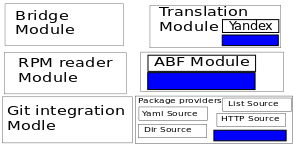
\includegraphics[width=10cm,height=10cm,keepaspectratio]{diagram.png}
\end{frame}

\begin{frame}
	\frametitle{Комментарии к архитектуре}
	\begin{enumerate}
		\item Можно добавить новые источники пакетов.
		\item Можно добавить новые средства машинного перевода.
		\item Можно интегрировать с другими системами, кроме ABF.
\end{enumerate}
\end{frame}


\begin{frame}
\frametitle{Планирование}

Пример в рамках одного из спринтов:

спринт длился 9 дней с 17.02 по 26.02. 

По плану:

- реализовать CLI-интерфейс (отв. Яковлев)

- реализовать динамическую подгрузку веток разработки (отв. Громов)

- реализовать GUI для импорта пакетов и машинного перевода строк (Ериков)

дедлайн на все 29.02.
\end{frame}
\begin{frame}
\frametitle{Планирование}

Реализовался риск - у Ерикова завал на работе, как следствие - к 26 GUI не был начат.

Выход из ситуации: смена технологий GUI с QT на Web scope, смена реализатора GUI.

Результат к 29.02:

- импорт пакетов и машинный перевод в GUI реализованы 

- CLI реализован

- по загрузке ветки уточнены требования у заказчика, задача отложена на следующий спринт.
\end{frame}

\begin{frame}
\frametitle{Проектирование - технологии}

Python - по желанию заказчика
PyQt - для связки GUI и Python
WevView для GUI в виду реализовавшегося риска
\end{frame}



\begin{frame}
\frametitle{Тестирование}

Тестирование проводилось в соответствии с ПМИ, а также по соответствию функциональным требованиям.
В результате были найдены и ликвидированы:

- ошибка загрузки и использования настроек
- ошибка формата машинного перевода в GUI
\end{frame}



\begin{frame}
	\frametitle{Выводы}
Разработанная программа позволяет экономить время при локализации пакетов под операционную систему Rosa Linux.
\end{frame}

\begin{frame}
\frametitle{Отзыв от заказчика}
В результате демонстрации программы, заказчик был удовлетворён функционалом продемонстрированного решения.

"Вполне похоже на то, что хотелось."



\end{frame}



\begin{frame}
	\frametitle{Демонстрация}
	
	Перейдем к программе...
\end{frame}


\begin{frame}[c]
\begin{center}
\frametitle{\LARGE Спасибо за внимание!}

{\LARGE \inserttitle}

\bigskip

{\insertauthor} 

\bigskip\bigskip

{\insertinstitute}

\bigskip\bigskip

{\large \insertdate}
\end{center}
\end{frame}
\end{document}
